%!TEX root = practicum1.tex
The parameter $K$ defines how hard the system is driven, that is why for $K = 0$ we would expect to have no perturbations. The trival case, $K = 0$, is discussed in \cref{ss:b:trivial}. 

As the value of $K$ increases we expect that the chaotic regions grow and eventually start to dominate the phase space \cite{finn200Cahaotic}. The effect of varying values of $K$ is discussed in \cref{ss:b:nontrivial}. 

Finally \cref{ss:b:kam} discusses KAM orbits in the context of the Chirikov map.

\subsubsection{Trivial Case}
\label{ss:b:trivial}
If we choose $K = 0$ \cref{eq:chirikov} becomes:
\begin{subequations}\label{eq:chirikovK0}
	\begin{align}
		\label{eq:chirikov0:p} p_{n + 1} &= p_n \mod 1,\\
		\label{eq:chirikov0:x} x_{n + 1} &= x_n + p_{n + 1} \mod 1.
	\end{align}
\end{subequations}	
Consequently the values of $p_n$ are constant for $n > 0$, since if $p_0 = 1$, then $p_1$ becomes zero as a consequence of the modulo operator in \eqref{eq:chirikov0:p}. This effect is illustrated by the horizontal lines in \cref{fig:experiment:fancy_k:0}. Additionally without the modulo in \eqref{eq:chirikov0:x}, $x_n$ would increase linearly, due to this operator however $x_n$ becomes periodic. 

\Cref{fig:experiment:K0influenceOfX} shows $x_0$ as a function of $n$ for a fixed value of $p_0$, if we compare the different plots  in this figure we observe that changing $x_0$ and fixing $p_0$ only influences the phase of $x_n$, and not the period. 

\begin{figure}[t]
	\centering
	\foreach \x/\actualX in {1/0.1, 3/0.3, 5/0.5}{
		\begin{subfigure}[t]{\columnwidth}
			\includegraphics[width=\textwidth]{./img/assignment_b_K=0p_0=04x_0=0\x.pdf}
			\caption{$x_0 = \actualX$}
			\label{fig:experiment:K0:X:\x}
		\end{subfigure}	
	}	
	\caption{$x_n$ as a function of $n$, for $p_0 = 0.4$,$K = 0$ and varying $x_0$.}
	\label{fig:experiment:K0influenceOfX}
\end{figure}

Fixing $x_0$ and varying $p_0$ results in \cref{fig:experiment:K0influenceOfP}, these plots show that $p_0$ influences the periodicity of the map, that is increasing $p_0$, increases the frequency of $x_n$.

\begin{figure}[t]
	\centering
	\foreach \p/\actualP in {1/0.1, 3/0.3, 5/0.5}{
		\begin{subfigure}[t]{\columnwidth}
			\includegraphics[width=\textwidth]{./img/assignment_b_K=0p_0=0\p x_0=04.pdf}
			\caption{$p_0 = \actualP$}
			\label{fig:experiment:K0:P:\p}
		\end{subfigure}	
	}	
	\caption{$x_n$ as a function of $n$, for $x_0 = 0.4$, $K = 0$ and varying $p_0$.}
	\label{fig:experiment:K0influenceOfP}
\end{figure}

\begin{figure*}
	\centering
	\foreach \k/\fnk in {0/0, 0.2/2, 0.4/4, 0.8/8, 1/10, 2/20, 3/30, 4/40}{
		\begin{subfigure}{0.32\textwidth}
			\centering
			\includegraphics[width=\textwidth]{./img/assignment_b_fancy_k_\fnk.jpg}
			\caption{$K = \k$}
			\label{fig:experiment:fancy_k:\fnk}
		\end{subfigure}
	}
	\begin{subfigure}{0.32\textwidth}
			\centering
			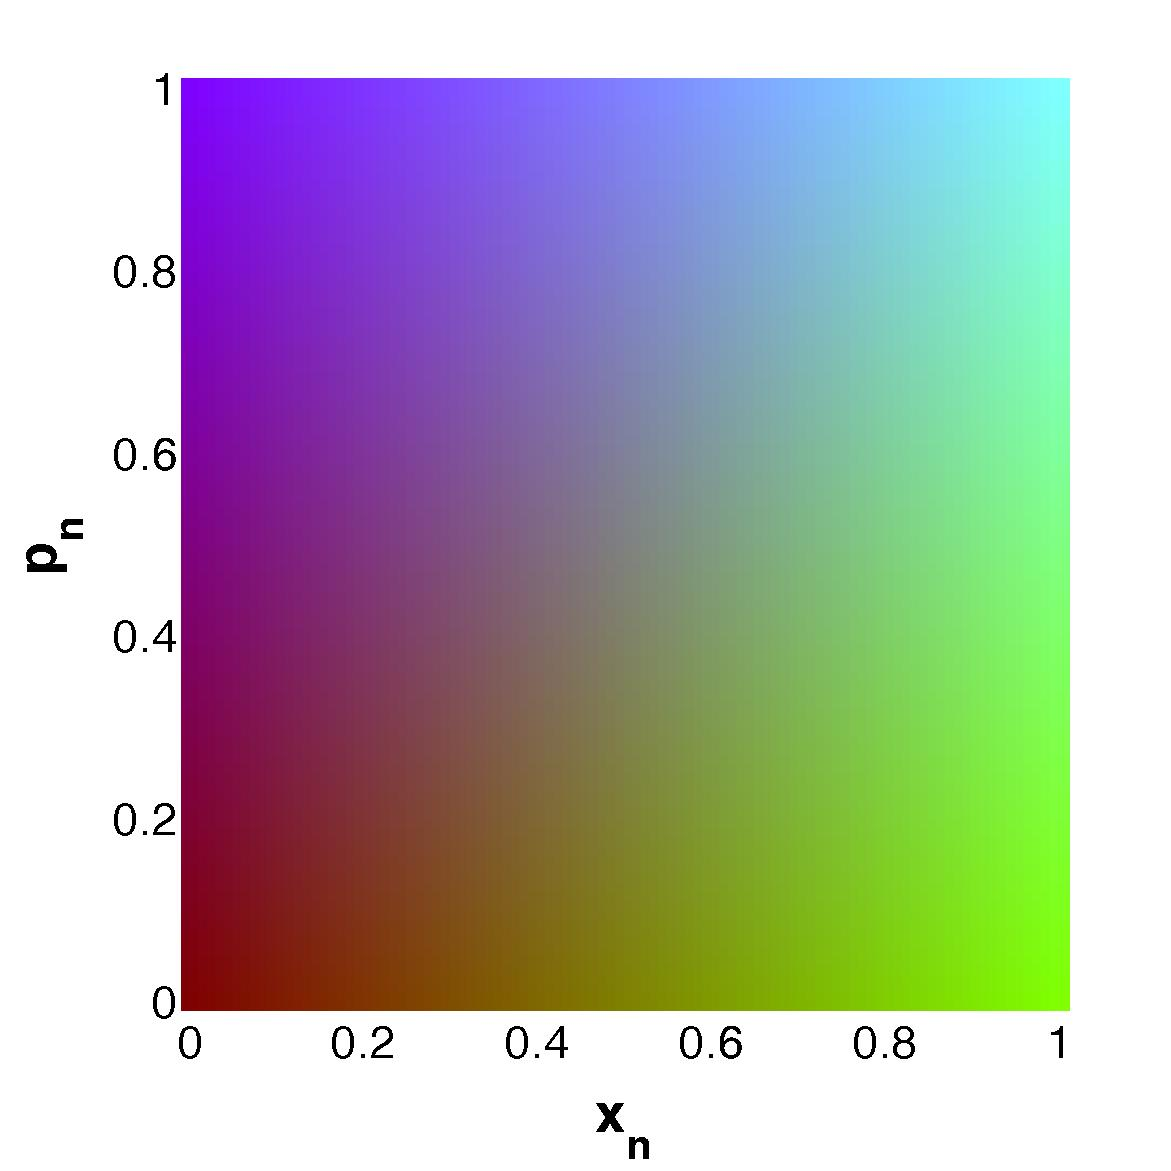
\includegraphics[width=\textwidth]{./img/assignment_b_colormap.jpg}
			\caption{Color map}
			\label{fig:experiment:fancy_k:colormap}
		\end{subfigure}
	\caption{$p_n$ (y-axis) as a function of $x_n$ (x-axis) for $p_0$ and $x_0$ in the unit square, $0 \leq n \leq 1000$ for different values of $K$. Each plot shows 100 Chirikov maps with random intiaisations of $x_0$ and $p_0$. \subref{fig:experiment:fancy_k:colormap} shows the colourmap for \subref{fig:experiment:fancy_k:0} through \subref{fig:experiment:fancy_k:40}.}
	\label{fig:experiment:fancy_k}
\end{figure*}

\begin{figure*}[ht]
	\centering
	\begin{subfigure}{0.32\textwidth}
		\centering
			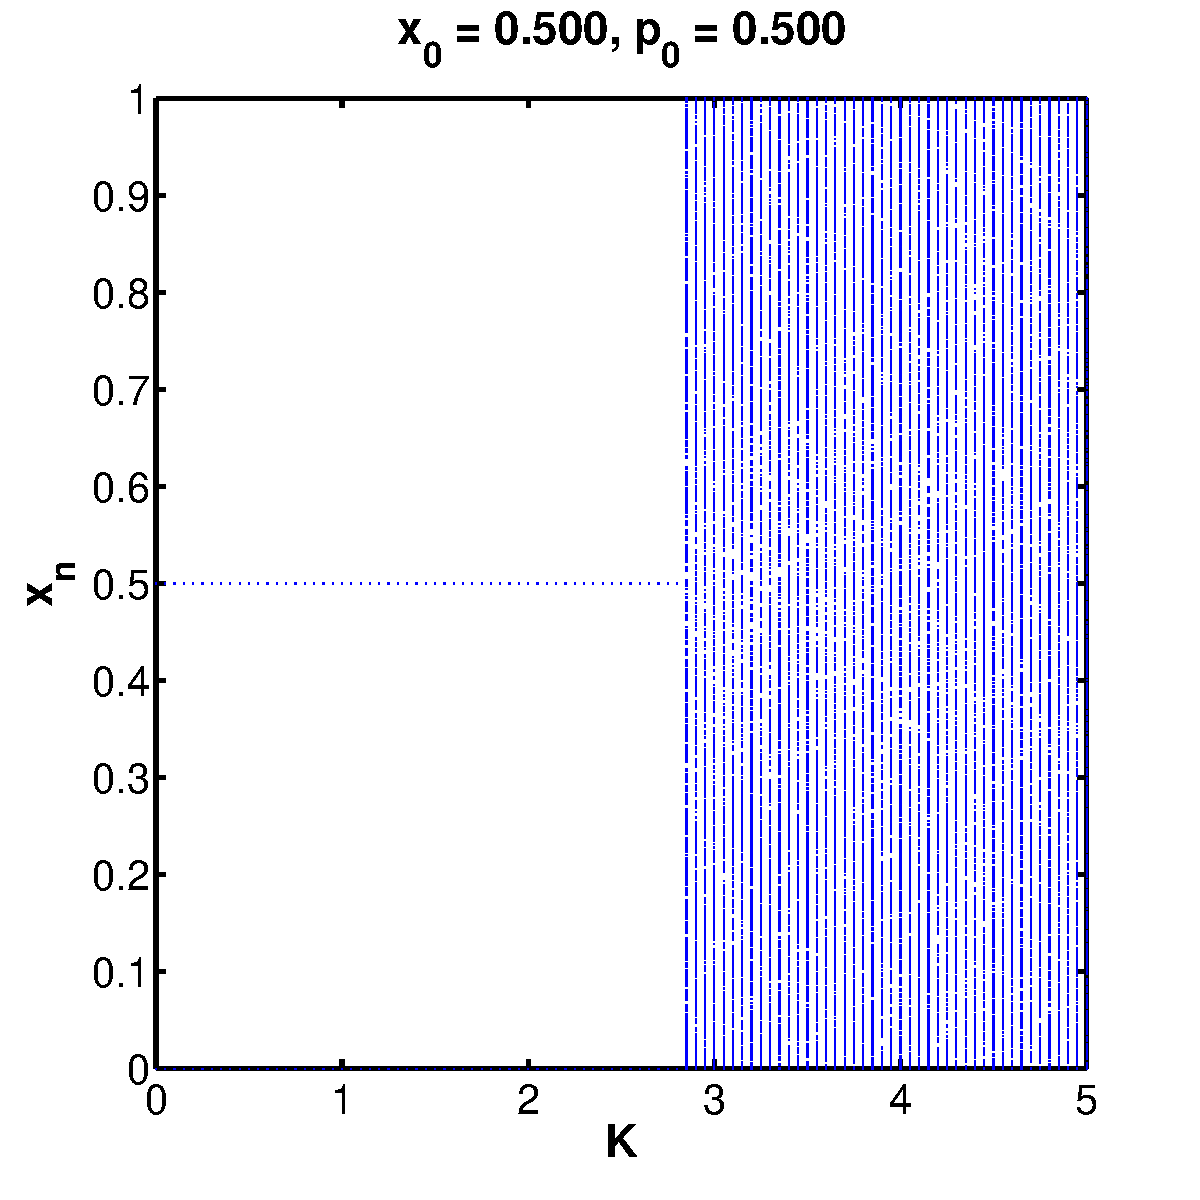
\includegraphics[width=\textwidth]{./img/assignment_b_dim_0_b_x}
			\caption{$x_0 = \num{0.6523678}$}
			\label{fig:experiment:bifurcation:x}
	\end{subfigure}
	\begin{subfigure}{0.32\textwidth}
		\centering
			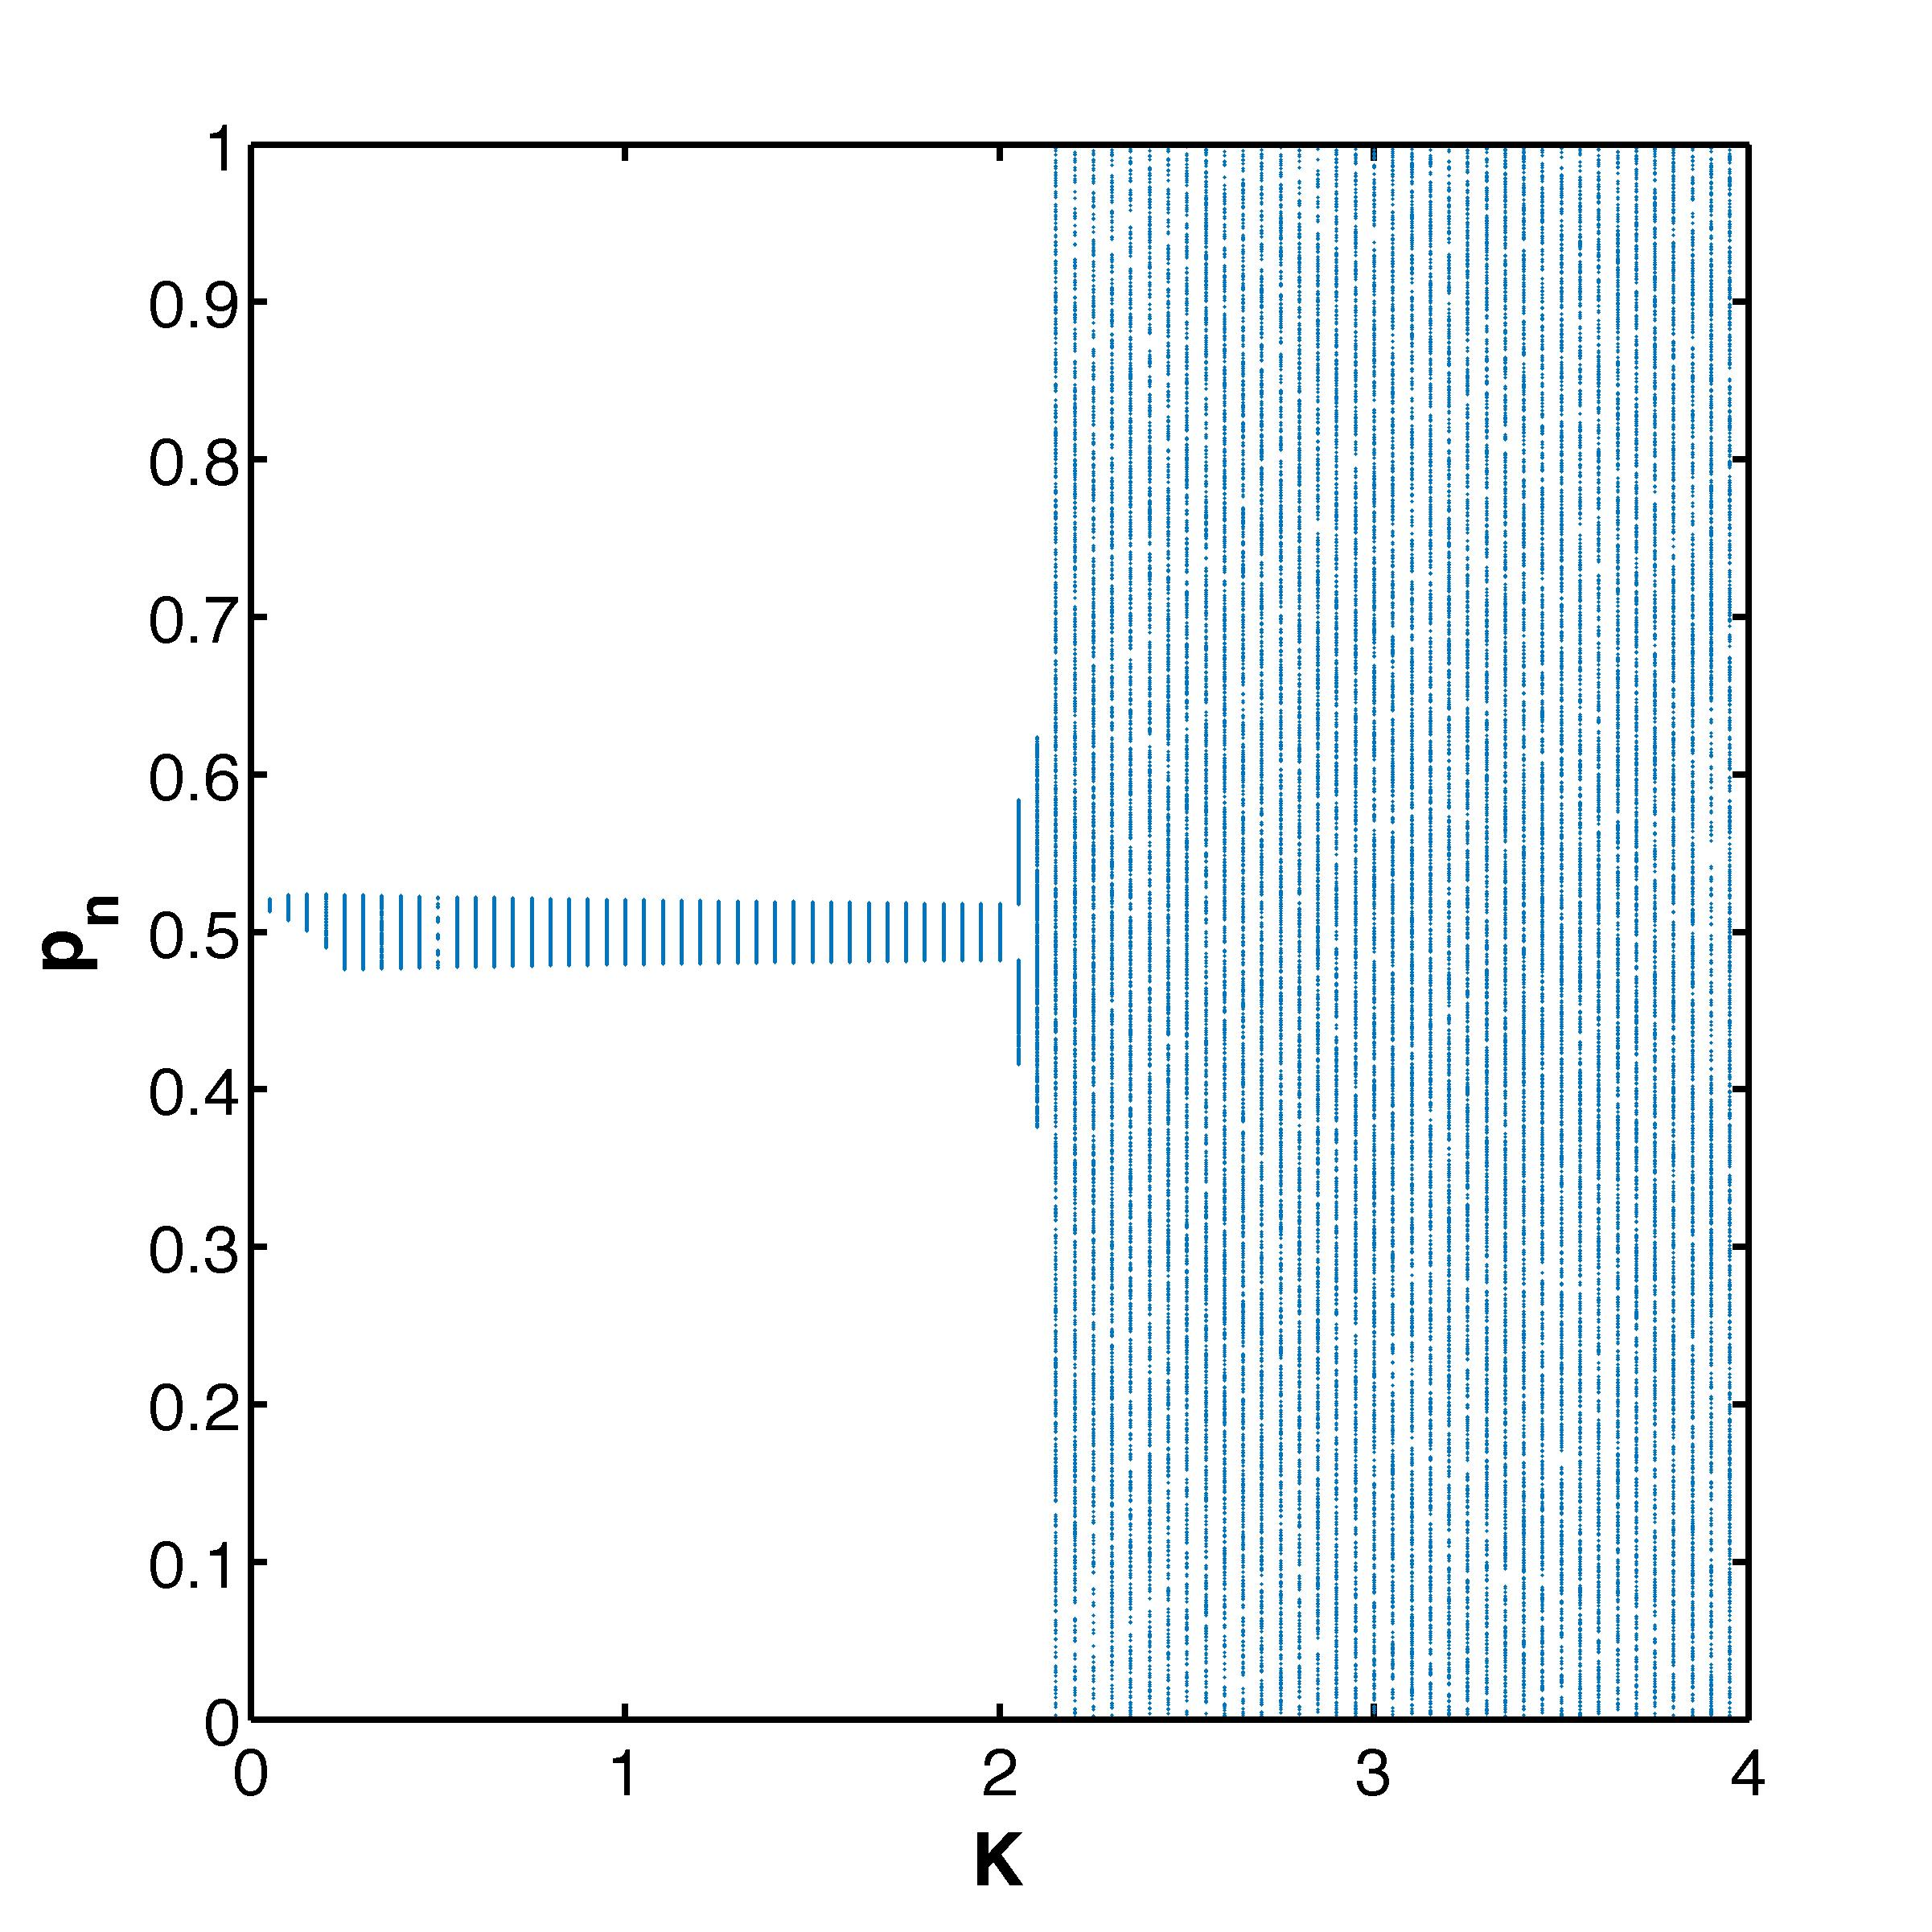
\includegraphics[width=\textwidth]{./img/assignment_b_dim_0_b_p}
			\caption{$p_0 = \num{0.0022312}$}
			\label{fig:experiment:bifurcation:p}
	\end{subfigure}
	\begin{subfigure}{0.32\textwidth}
		\centering
			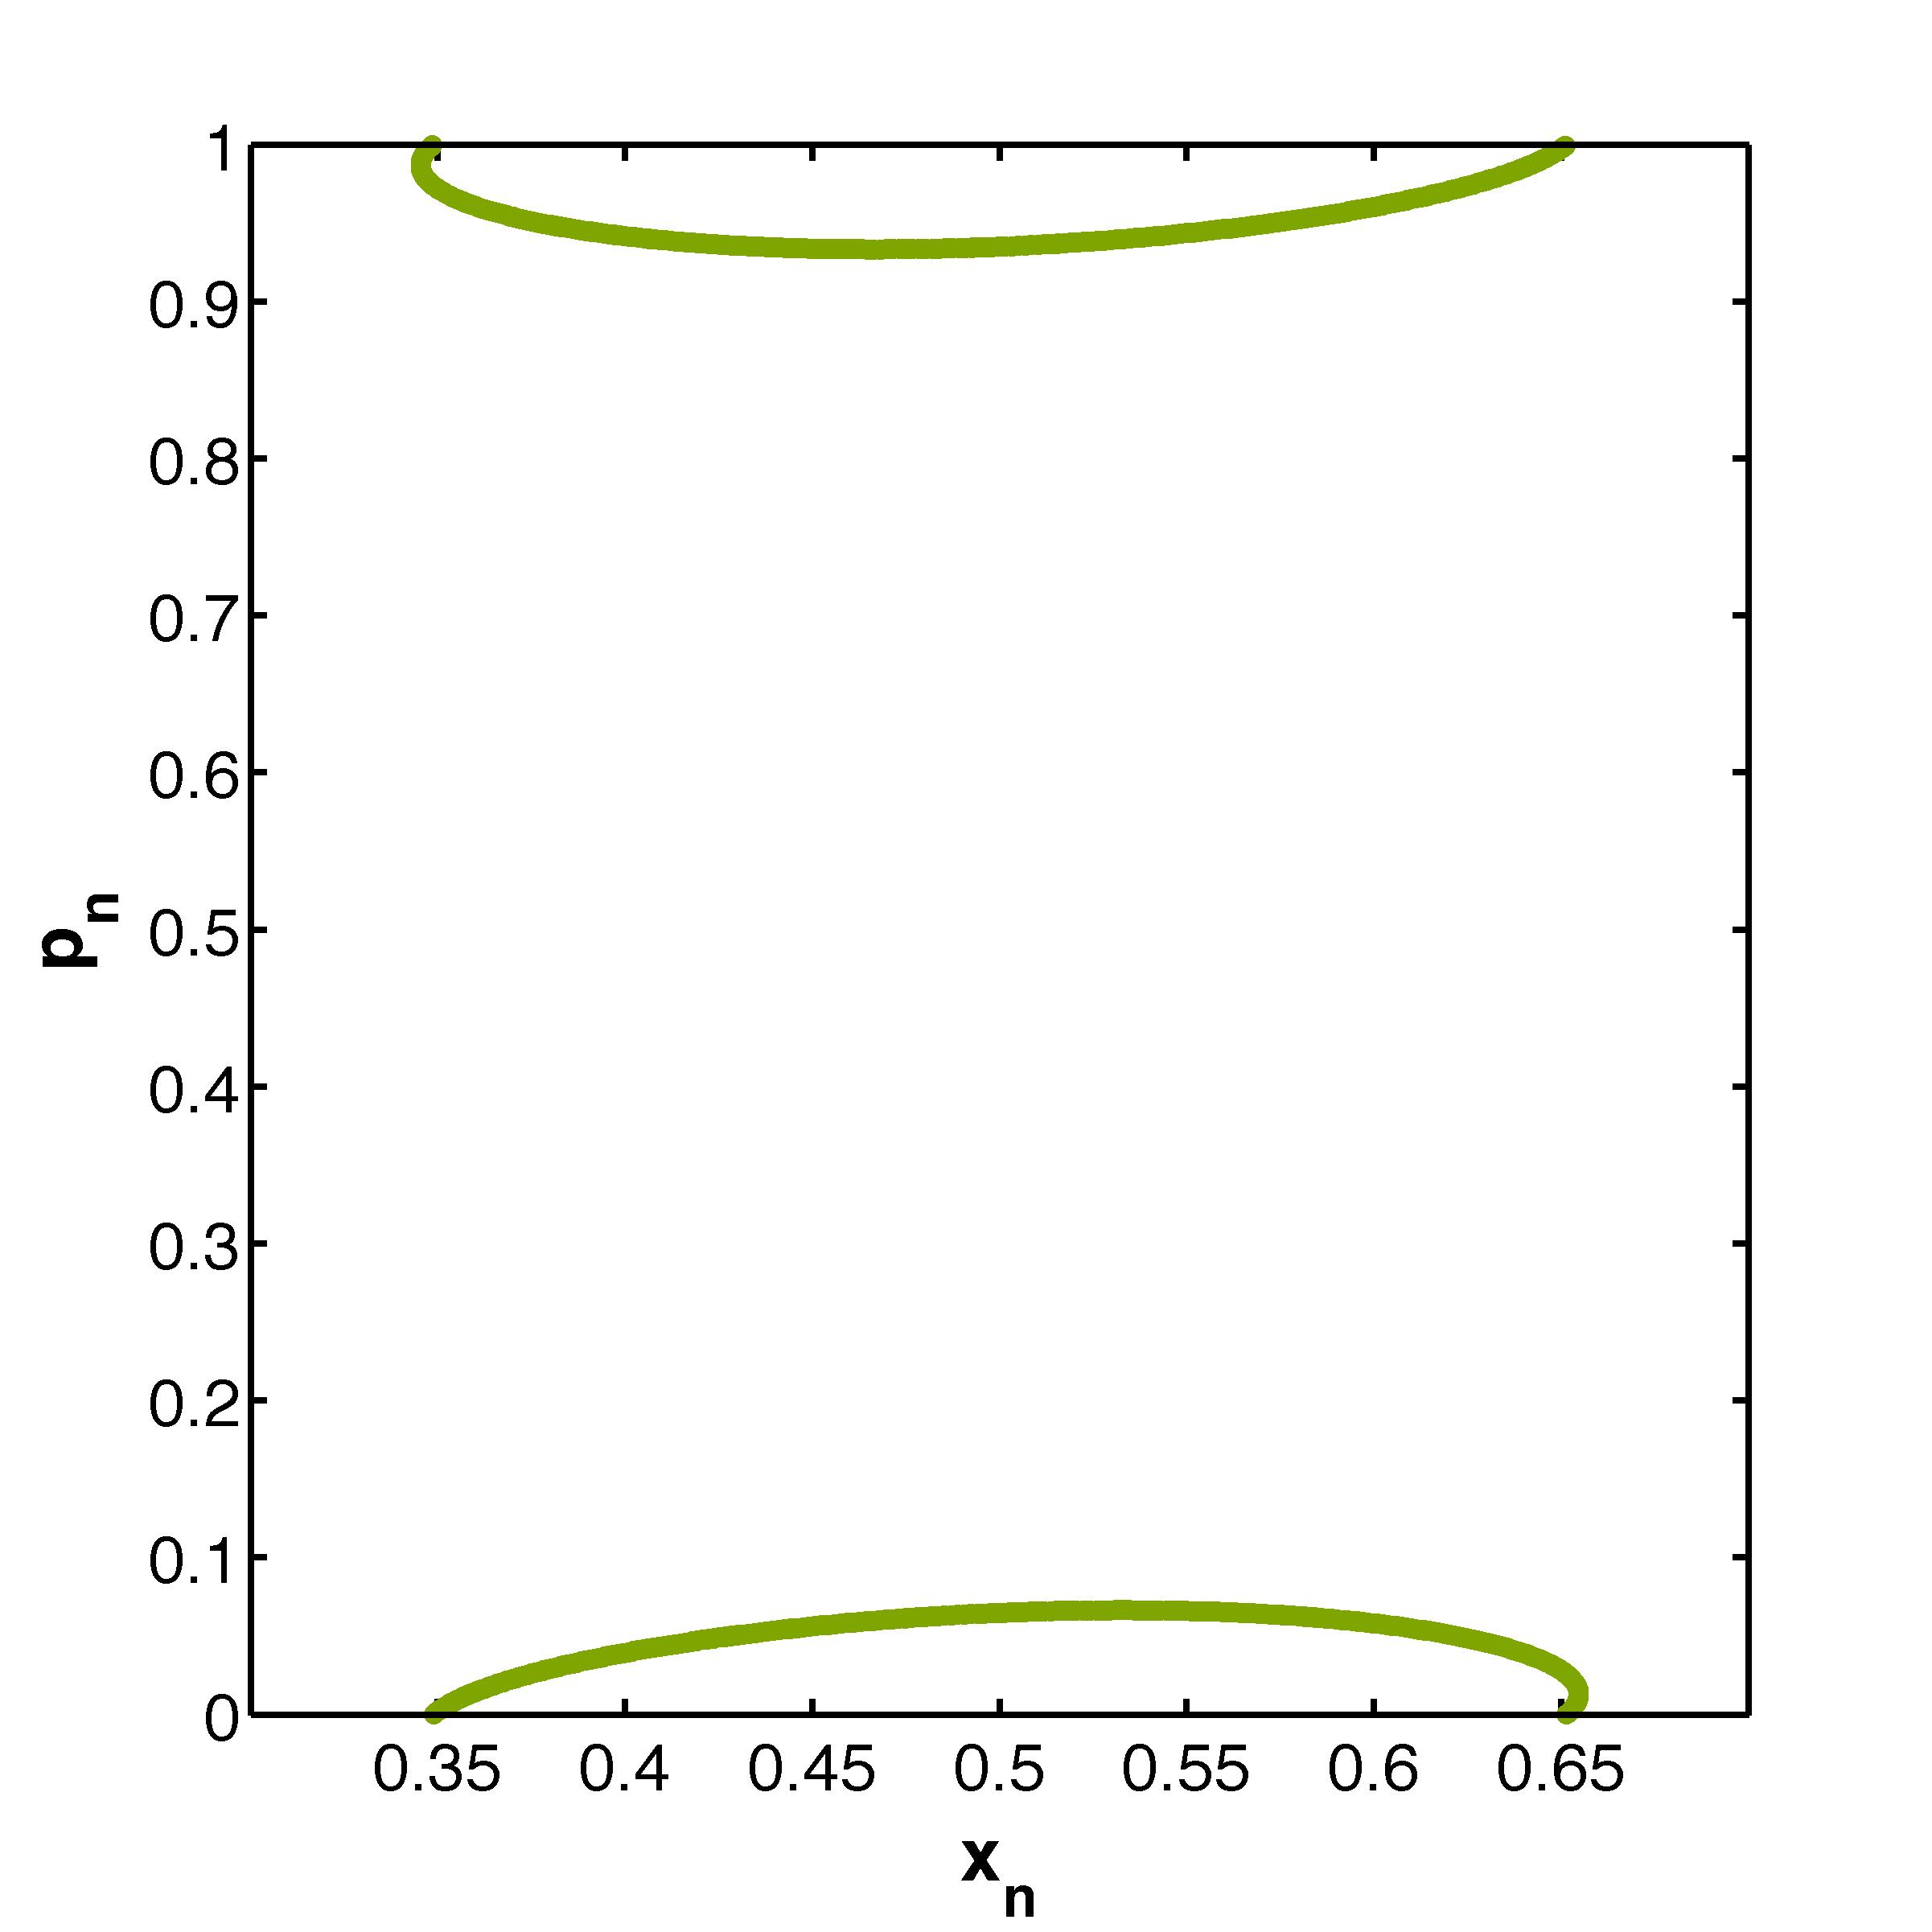
\includegraphics[width=\textwidth]{./img/assignment_b_bfp_orbit}
			\caption{The orbit ($K = 0.2$)}
			\label{fig:experiment:bifurcation:orbit}
	\end{subfigure}
	\caption{Bifurcation plots and corresponding orbit for $x_0 = \num{0.6523678}$ and $p_0 = \num{0.0022312}$ to illustrate the period doubling like effect.}
	\label{fig:experiment:bifurcation}
\end{figure*}

\subsubsection{Non-Trivial Case}
\label{ss:b:nontrivial}
\todo[inline]{How do the orbits change with increasing K? Do we have scenarios that are similar to period doubling? Done at least a bit.}
\Cref{fig:experiment:fancy_k} shows the influence of variable $K$. As noted before $K$ determines the drive of the system resulting in more chaotic behaviour with a higher $K$. The images in \cref{fig:experiment:fancy_k} were created by plotting 100 Chirikov maps with randomly chosen values for $x_0$ and $p_0$. The colour for each map was determined by its initialisation. The mapping from the colours to the initial values are shown in \cref{fig:experiment:fancy_k:colormap}. Due to this mapping of colours we can see that up until $K = 1$ the colours stay in the same order, as opposed to $K = 2$ to $K = 4$ were this order is completely gone.

We consider a phase space to be more chaotic when there are more or bigger filled areas in the images. As can be expected from the discussion in our previous section the map created with $K = 0$ shows only horizontal lines, with fits with the constant $p_n$. Interesting is the difference in line types i.e. there are filled and dotted lines, indicating different periods for $x_n$. Note that the \textit{resolution} of the map is important when looking at these maps as an illustration. I.e. some dashed line may appear to be solid line because of the choice of point size and scale of the illustration. Also the maps shown in this paper were created using a finite number of steps. It might be the case that some high frequency periodic behaviour converges to one period when more steps are calculated.

At $K = 0.2$ we see that some of the horizontal lines from \cref{fig:experiment:fancy_k:0} are replaced by closed curves in the upper and lower part of the image, see \cref{fig:experiment:fancy_k:2}. Because the colours in the image map to initial values we see that the curves that appear in the upper and lower part have approximately the same initial values. This resembles a kind of period doubling. \Cref{fig:experiment:bifurcation} shows this period doubling like behaviour in a bifurcation diagram, together with the corresponding orbit which resembles the one we described.

In \Cref{fig:experiment:fancy_k:8} we can see that chaos increases ($K = 0.8$), as some regions are already starting to be filled in by two-dimensional orbits, they are especially noticeable in the corners of the plot.

 Finally in the images shown in \cref{fig:experiment:fancy_k:20} - \ref{fig:experiment:fancy_k:40} we see that the chaotic orbits start to completely dominate the image. With in the last two images (\cref{fig:experiment:fancy_k:30} and \ref{fig:experiment:fancy_k:40}) only a few stable initialisations left. 

\subsubsection{KAM-orbits}
\label{ss:b:kam}
\citeauthor{kenzel1997physics} define Kolmogorov-Arnold-Moser-orbits as one-dimensional orbits that traverse the entire phase-state diagram horizontally. These KAM orbits are represented by the solid lines in  \cref{fig:experiment:fancy_k}. Looking closely at \cref{fig:experiment:fancy_k:0} we observe that not all orbits are $KAM$-orbits, since some of the lines are clearly dashed. Note that here the \textit{resolution problem}, as discussed in the previous section, also has to be considered. An interesting property of the KAM-orbits is that it can be shown that chaotic orbits cannot cross the one-dimensional orbits \cite{kenzel1997physics}. Consequently they restrict the extent of the chaos of the two-dimensional orbits.\\

\begin{figure}
	\centering
	\begin{subfigure}{\columnwidth}
		\centering
		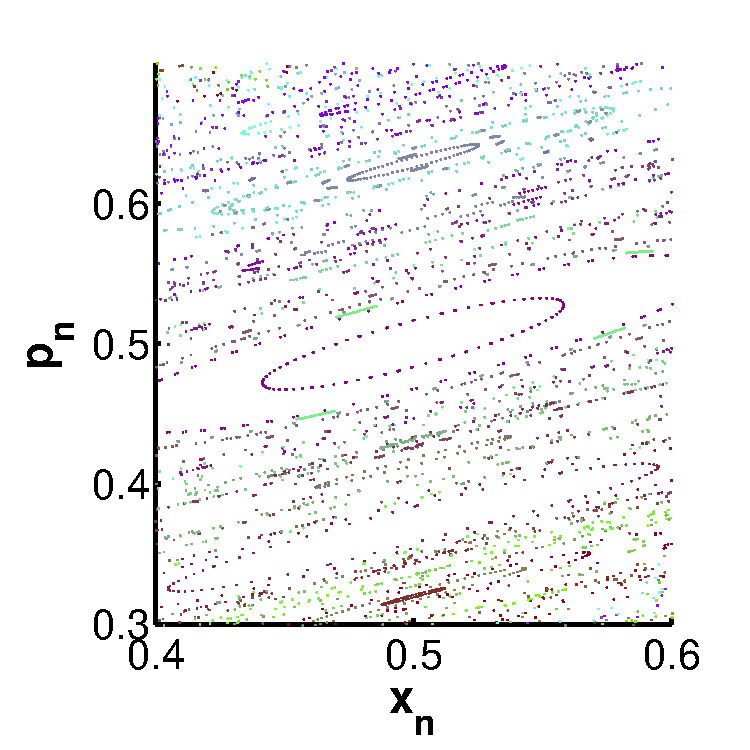
\includegraphics[width=\textwidth]{./img/assignment_b_fancy_k_9700}
		\caption{$K = 0.970000$}
		\label{fig:experiment:b:96}
	\end{subfigure}
	\begin{subfigure}{\columnwidth}
		\centering
		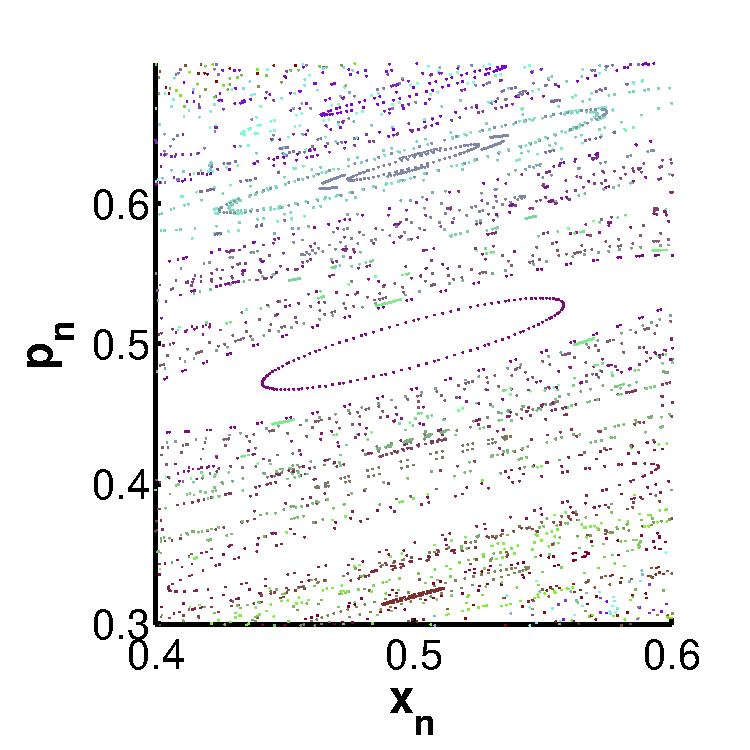
\includegraphics[width=\textwidth]{./img/assignment_b_fancy_k_9716}
		\caption{$K = K_c$}
		\label{fig:experiment:b:KC}
	\end{subfigure}	
	\caption{$p_n$ as a function of $x_n$ for $0.4 \leq x_n \leq 0.6$, $0.3 \leq p_n \leq 0.7$ and $0 \leq n \leq 250$. \subref{fig:experiment:b:96} show the phase-state diagram for $K = 0.970000$ and \subref{fig:experiment:b:KC} for $K = K_c$. The 200 initial values for $p$ and $x$ where chosen randomly, but were identical for both values of $K$.}
	\label{fig:experiment:b:testKC}
\end{figure}

\citeauthor{greene1979method} observed that for small values of $K$ there are many KAM orbits that encircle the islands horizontally, see \cref{fig:experiment:fancy_k:0}, \ref{fig:experiment:fancy_k:2} and \ref{fig:experiment:fancy_k:4}. These KAM orbits divide the space into several compartments which may contain chaotic orbits. For larger values of $K$ there are fewer KAM orbits and individual chaotic orbits occur a greater are of the phase space. Finally at some critical value of $K$, called $K_c$, the last KAM orbit disappears, this effect can be observed in \cref{fig:experiment:fancy_k:10}. 

It has been found that for $K < K_c = 0.971635\dotsc$, one-dimensional-orbits exist that traverse the entire phase-state diagram horizontally \cite{kenzel1997physics}. If we plot the phase-state diagram for a value of $K$ that is slightly smaller than $K_c$, \cref{fig:experiment:b:96}, and for $K = K_c$, \cref{fig:experiment:b:KC}, we observe that the single KAM-orbit in \cref{fig:experiment:b:96} has disappeared in \cref{fig:experiment:b:KC}. 

